\newpage

\subsection{QuizziPedia::Front-End::ModelViews}
\subsubsection{Informazioni generali}
\label{QuizziPedia::Front-End::ModelViews}
\begin{figure}
	\centering
	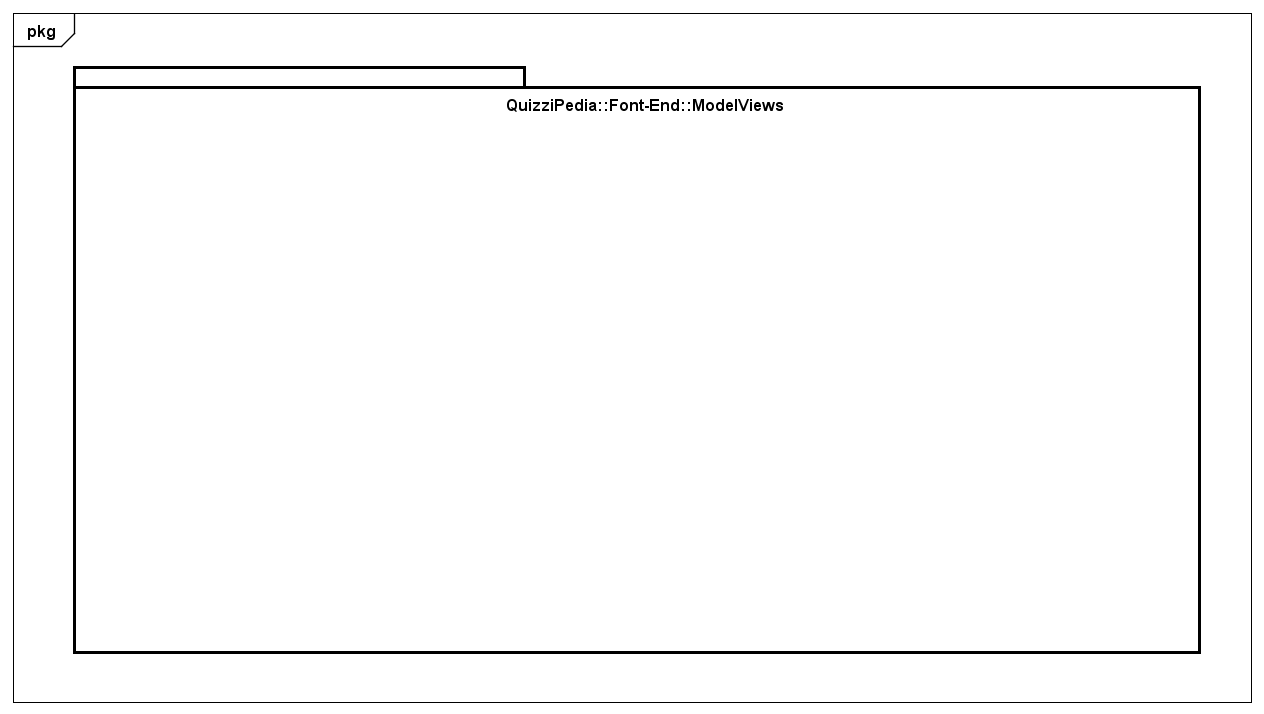
\includegraphics[scale=0.45]{UML/Package/QuizziPedia_Front-End_ModelViews.png}
	\caption{QuizziPedia::Front-End::ModelViews}
\end{figure}
\begin{itemize}
	\item \textbf{Descrizione}: ;
	\item \textbf{Padre}: \texttt{Front-End};
	\item \textbf{Interazione con altri componenti}:
	\begin{itemize}
		\item \texttt{Controllers}: package contenente i controllers front-end dell'applicazione;
		\item \texttt{Directives}: package contenente le directives front-end dell'applicazione;
		\item \texttt{View}: .
	\end{itemize}
\end{itemize}
\subsubsection{Classi}


